\begin{frame}[t]{Wheatstone Bridge}

  Die Wheatstone Bridge ist eine einfache Schaltung um einen Wiederstand zu messen. Die Schaltung gilt als abgeglichen, wenn an $V_{AB}$ keine Spannng anliegt.

  Die theoretische Herleitung ist nicht ganz trivial, daher möchten wir an dieser Stelle die Realität und den Aufwand eines praktischen Aufbaus der Flexibilität einer Simulation gegenüberstellen.


  \begin{figure}
    \scalebox{0.6}{
      \centering
      \begin{circuitikz}
        \ctikzset{bipoles/thickness=1}
        \ctikzset{bipoles/length=.6cm}
        \draw
        (0,0) to [short, *-] (4,0)
        (0,0) to [V, l_=$V_{1}$] (0,-4)
        (2,0) to (2,-0.5)
        (4,0) to (4,-0.5)
        (2,-0.5) to [R, l_=$R_{1}$] (2,-1.5)
        (2,-2.5) to [R, l_=$R_{2}$] (2,-3.5)
        (2,-1.5) to (2,-2.5)
        (2,-2) to [short,*-o] (2.25,-2) node[right]{$V_{a}$}
        (4,-1.5) to (4,-2.5)
        (4,-2) to [short,*-o] (4.25,-2) node[right]{$V_{b}$}
        (4,-0.5) to [R, l_=$R_{3}$] (4,-1.5)
        (4,-2.5) to [R, l_=$R_{4}$] (4,-3.5)
        (2,-3.5) to (2,-4)
        (4,-3.5) to (4,-4)
        (0,-4) node[ground]{}
        (2,-4) node[ground]{}
        (4,-4) node[ground]{}
        ;
      \end{circuitikz}
    }
  \end{figure}

\end{frame}

\begin{frame}[t]{Experiment}

  Wir werden jetzt den folgenden Aufbau "live" analysieren. Beachtet, dass die Schaltung komplexer ist als in dem einleitenden schematischen Aufbau - wie immer.

  \begin{spacing}{0.9} \begin{tiny}
      \begin{minipage}{\textwidth}
        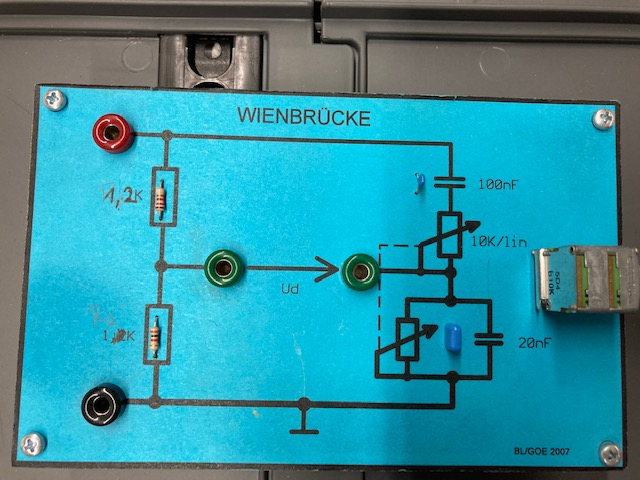
\includegraphics[width=0.5\linewidth]{pictures/wheatstone_bridge.jpg}
      \end{minipage}
    \end{tiny} \end{spacing}

  \textbf{Leitet aus der gemessenen Spannung den Wiederstandswert her.}

\end{frame}


\begin{frame}[t]{Simulation - Vorgehen}

  Wir wollen die Wienbrücke bei einer festen Spannungsversorgung $Sine(0\ 1\ 5k)$ abgleichen.
  \begin{itemize}
    \item Hierfür variieren wir den Trimmer bis die Differenzspannung $U_{AB}$ null beträgt.
    \item Via LTspice können wir uns dem abgeglichen Zustand annähern, indem wir den Trimmer als Variable betrachten.
    \item Hierfür nutzen wir die Variable $RT$ mit der Spice directive $.step\ param\ RT\ Anfangswert\ Endwert\ Inkrement$ und tasten uns an die ideale Trimmereinstellung heran.
    \item Mittels der Funktion select steps ermitteln wir die am besten abgeglichen Widerstände und passen unsere Variable sukzessive an.
  \end{itemize}

\end{frame}

\begin{frame}[t]{Simulation - Transient}

  Bitte baut die unten stehende Schaltung nach und führt das Experiment durch.

  \begin{spacing}{0.9} \begin{tiny}
      \begin{minipage}{\textwidth}
        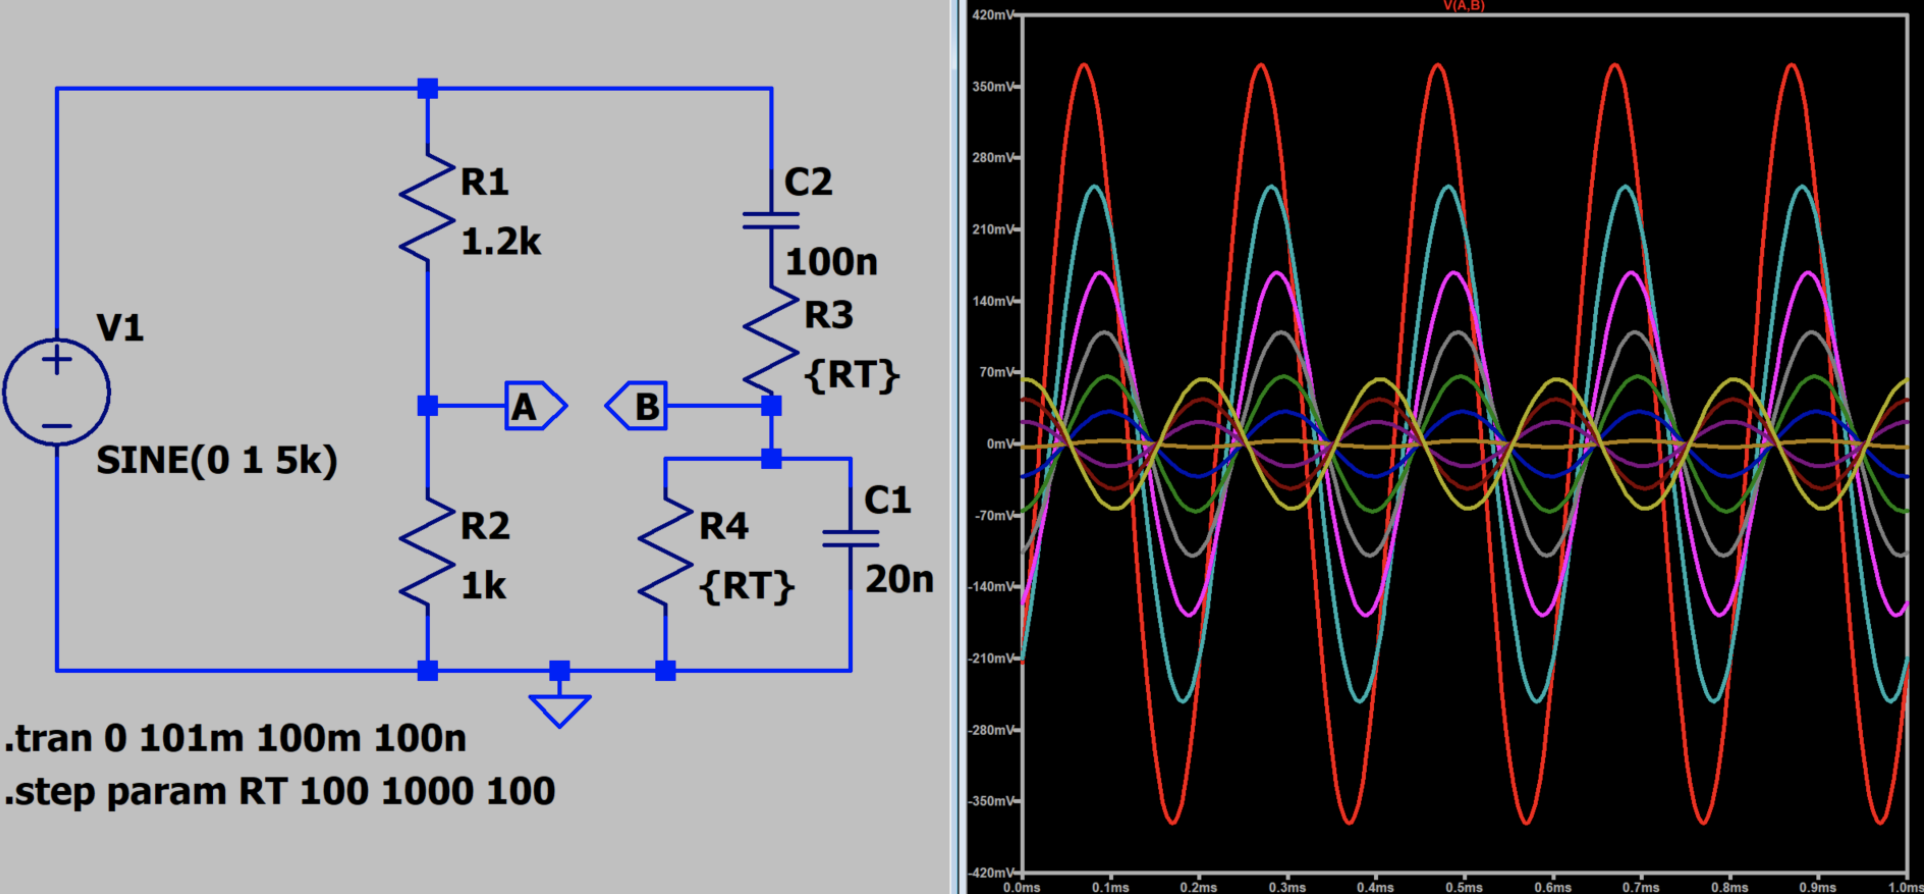
\includegraphics[width=0.75\linewidth]{pictures/wheatstone_simulation.png}
      \end{minipage}
    \end{tiny} \end{spacing}

  \textbf{Bei etwa $7120\Omega$ ist die Brücke abgeglichen - wir ersetzen die Variable durch einen festen Widerstandswert.}

\end{frame}

\begin{frame}[t]{Simulation - AC}

  Simulieren wir nun das Verhalten über die Frequenz via AC Analysis.

  \begin{spacing}{0.9} \begin{tiny}
      \begin{minipage}{\textwidth}
        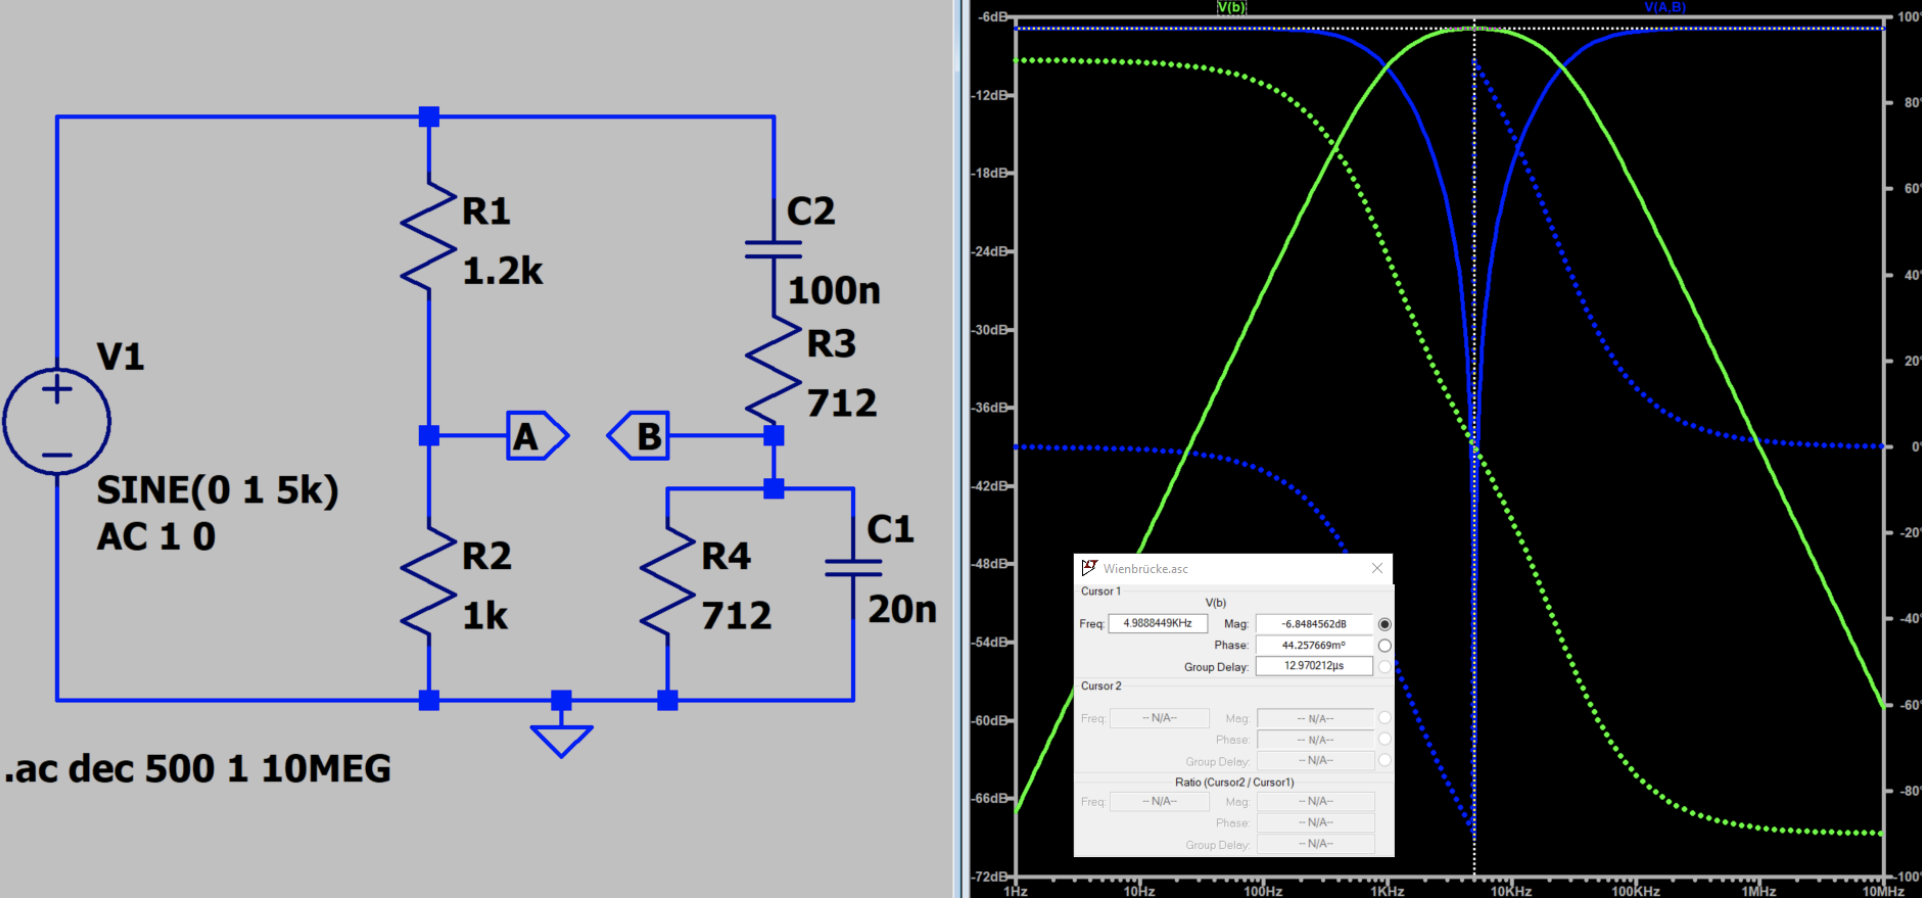
\includegraphics[width=0.75\linewidth]{pictures/wheatstone_ac.png}
      \end{minipage}
    \end{tiny} \end{spacing}

\end{frame}

\begin{frame}[t]{Simulation - AC Analyse}

  Betrachten wir zunächst die Spannung $U_A$, bzw. $U_B$.

  \begin{itemize}
    \item Im rechten Teilzweig der Schaltung ergibt sich durch den in Reihe verbauten Tiefpass und Hochpass ein Bandpassverhalten.
    \item Lediglich in einem mittleren Frequenzbereich um 5kHz ergibt sich eine Spannung $U_{AB}$.
  \end{itemize}

  Hieraus resultiert ein umgekehrtes Verhalten der Differenzspannung $U_{AB}$. Hier zeigt sich das Verhalten einer Bandsperre.
  Die Differenzspannung $U_{AB}$ ist bei 5kHz ideal abgeglichen und die Spannungen $U_{A}$ und $U_{B}$ heben sich gegenseitig auf.
\end{frame}

\begin{frame}[t]{Simulation - AC Grenzfrequenzen}

  Die Schaltung hat ja nach Betrachtung ein Bandpass- bzw. Bandsperrverhalten. Wir bestimmen die Grenzfrequenzen für beiden Messpunkte, $U_A$ und $U_{AB}$.
  \begin{itemize}
    \item $U_A$ Bandpass - \textbf{977 kHz}
    \item $U_{AB}$ Bandsperre - \textbf{977 kHz}
  \end{itemize}

  \begin{figure}
    \centering
    \subfloat{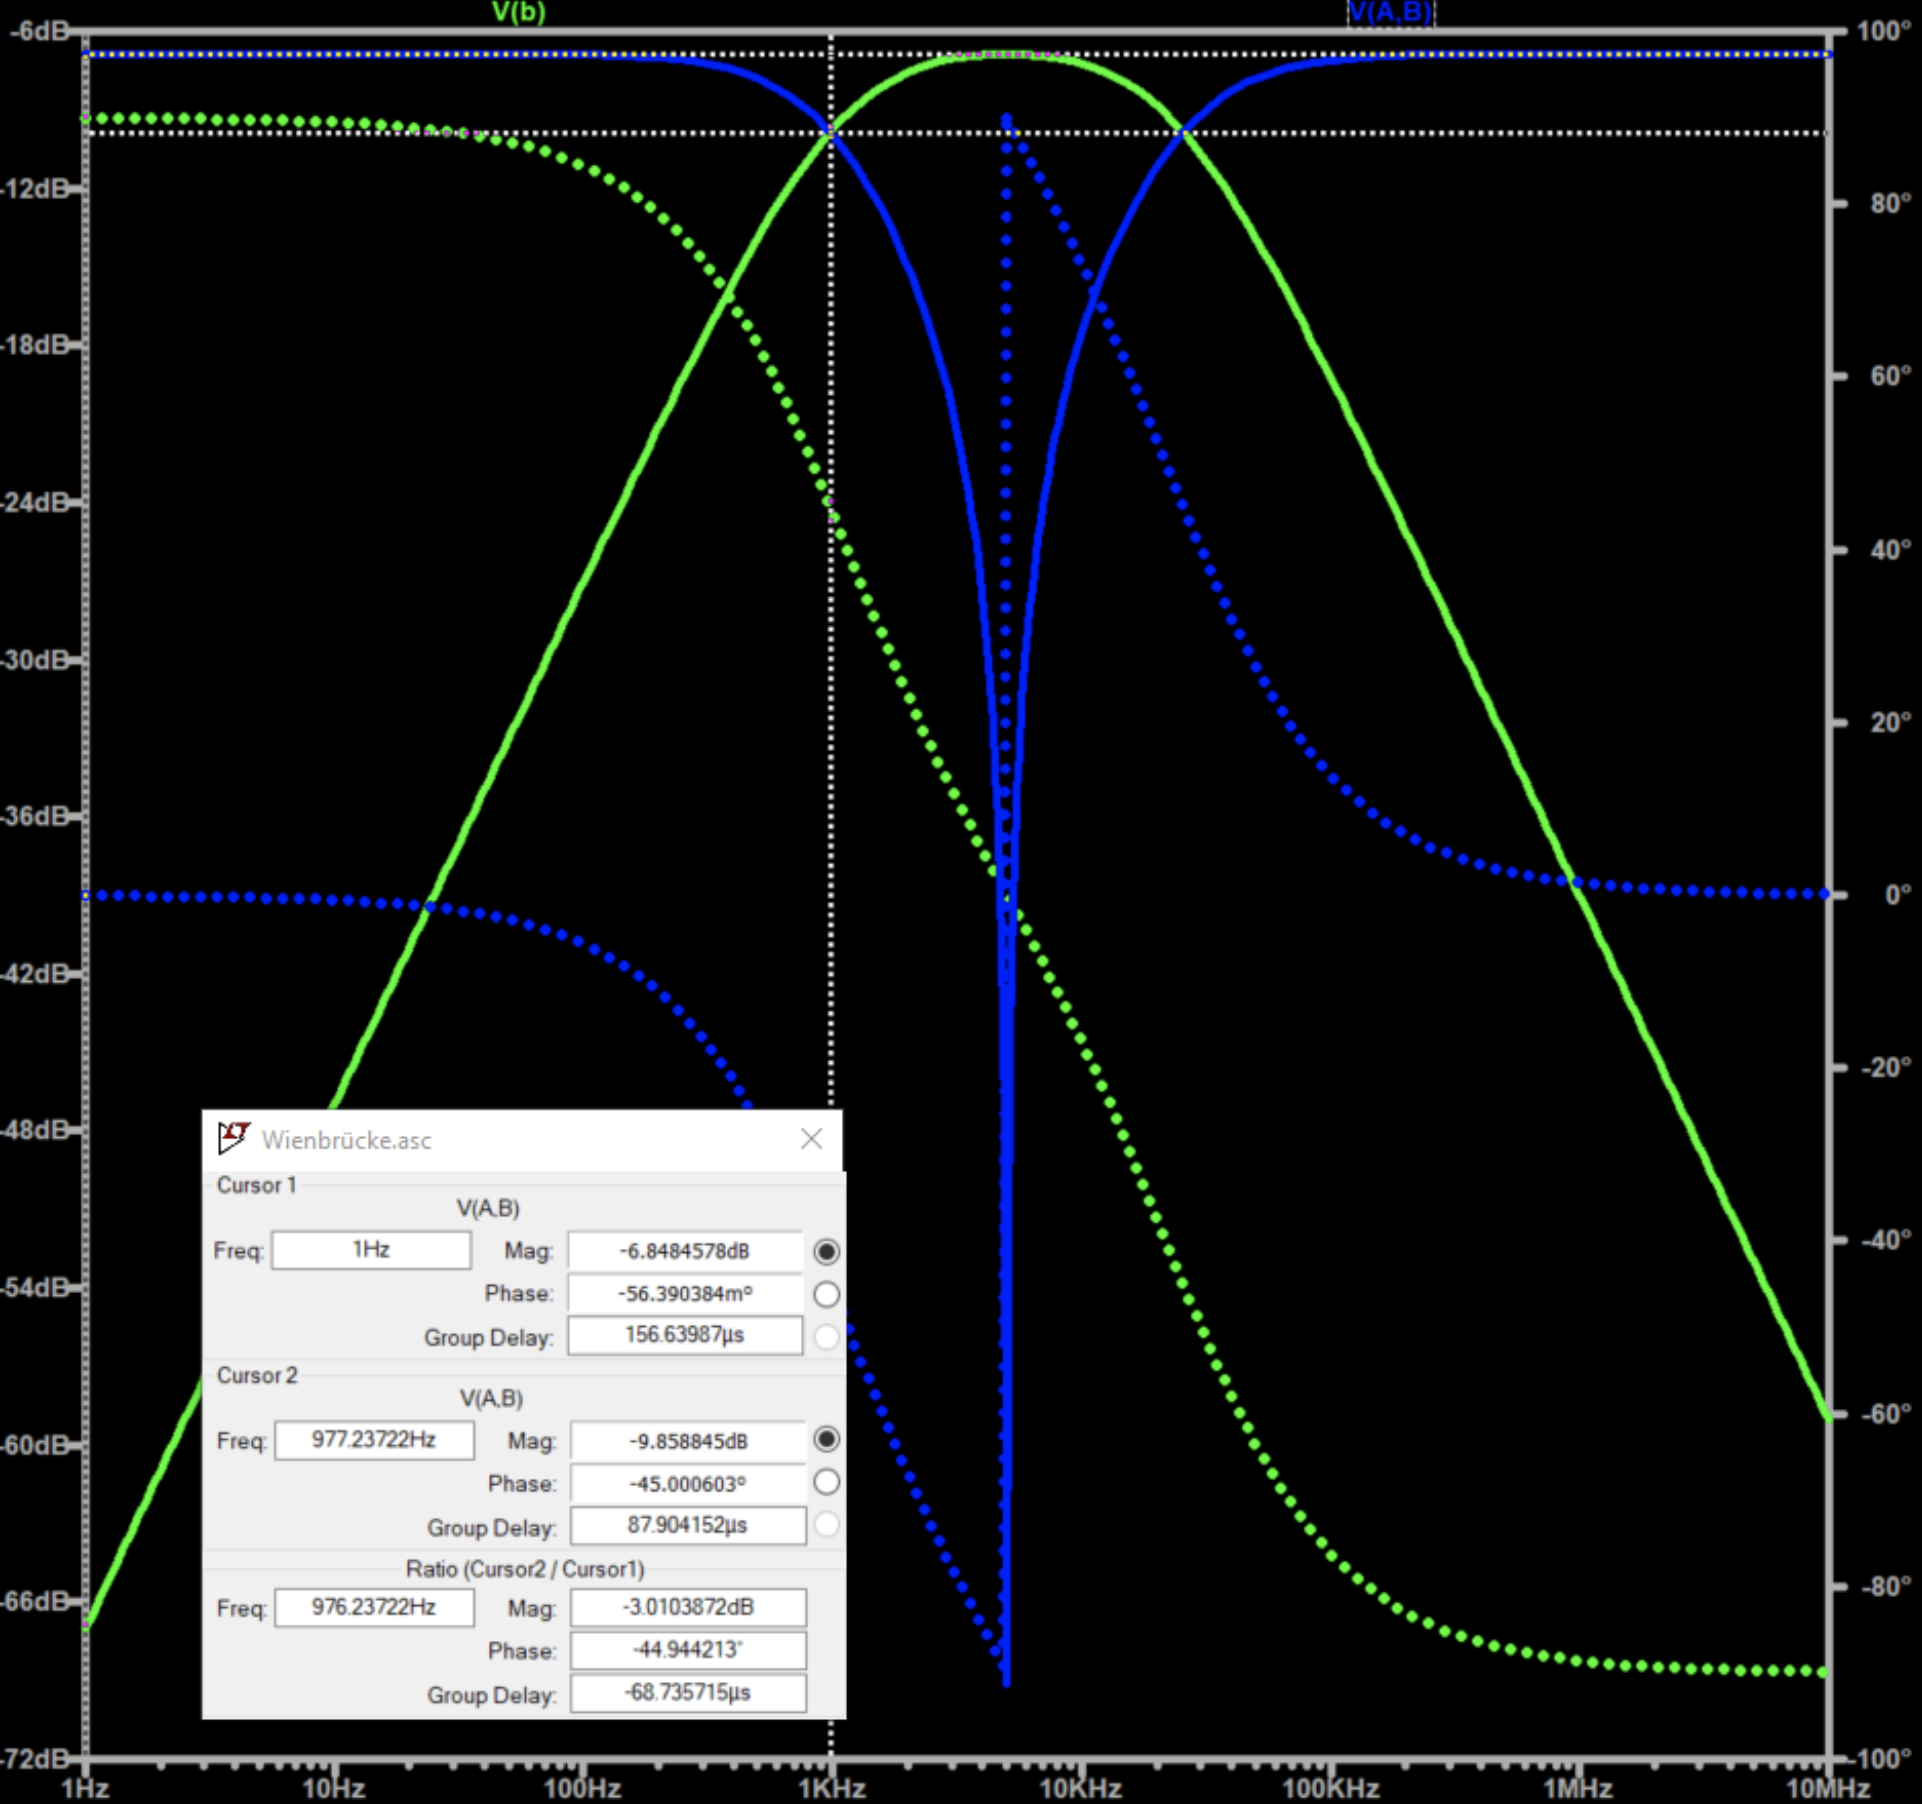
\includegraphics[width=4.5cm]{pictures/Bandpass.png}}\qquad
    \subfloat{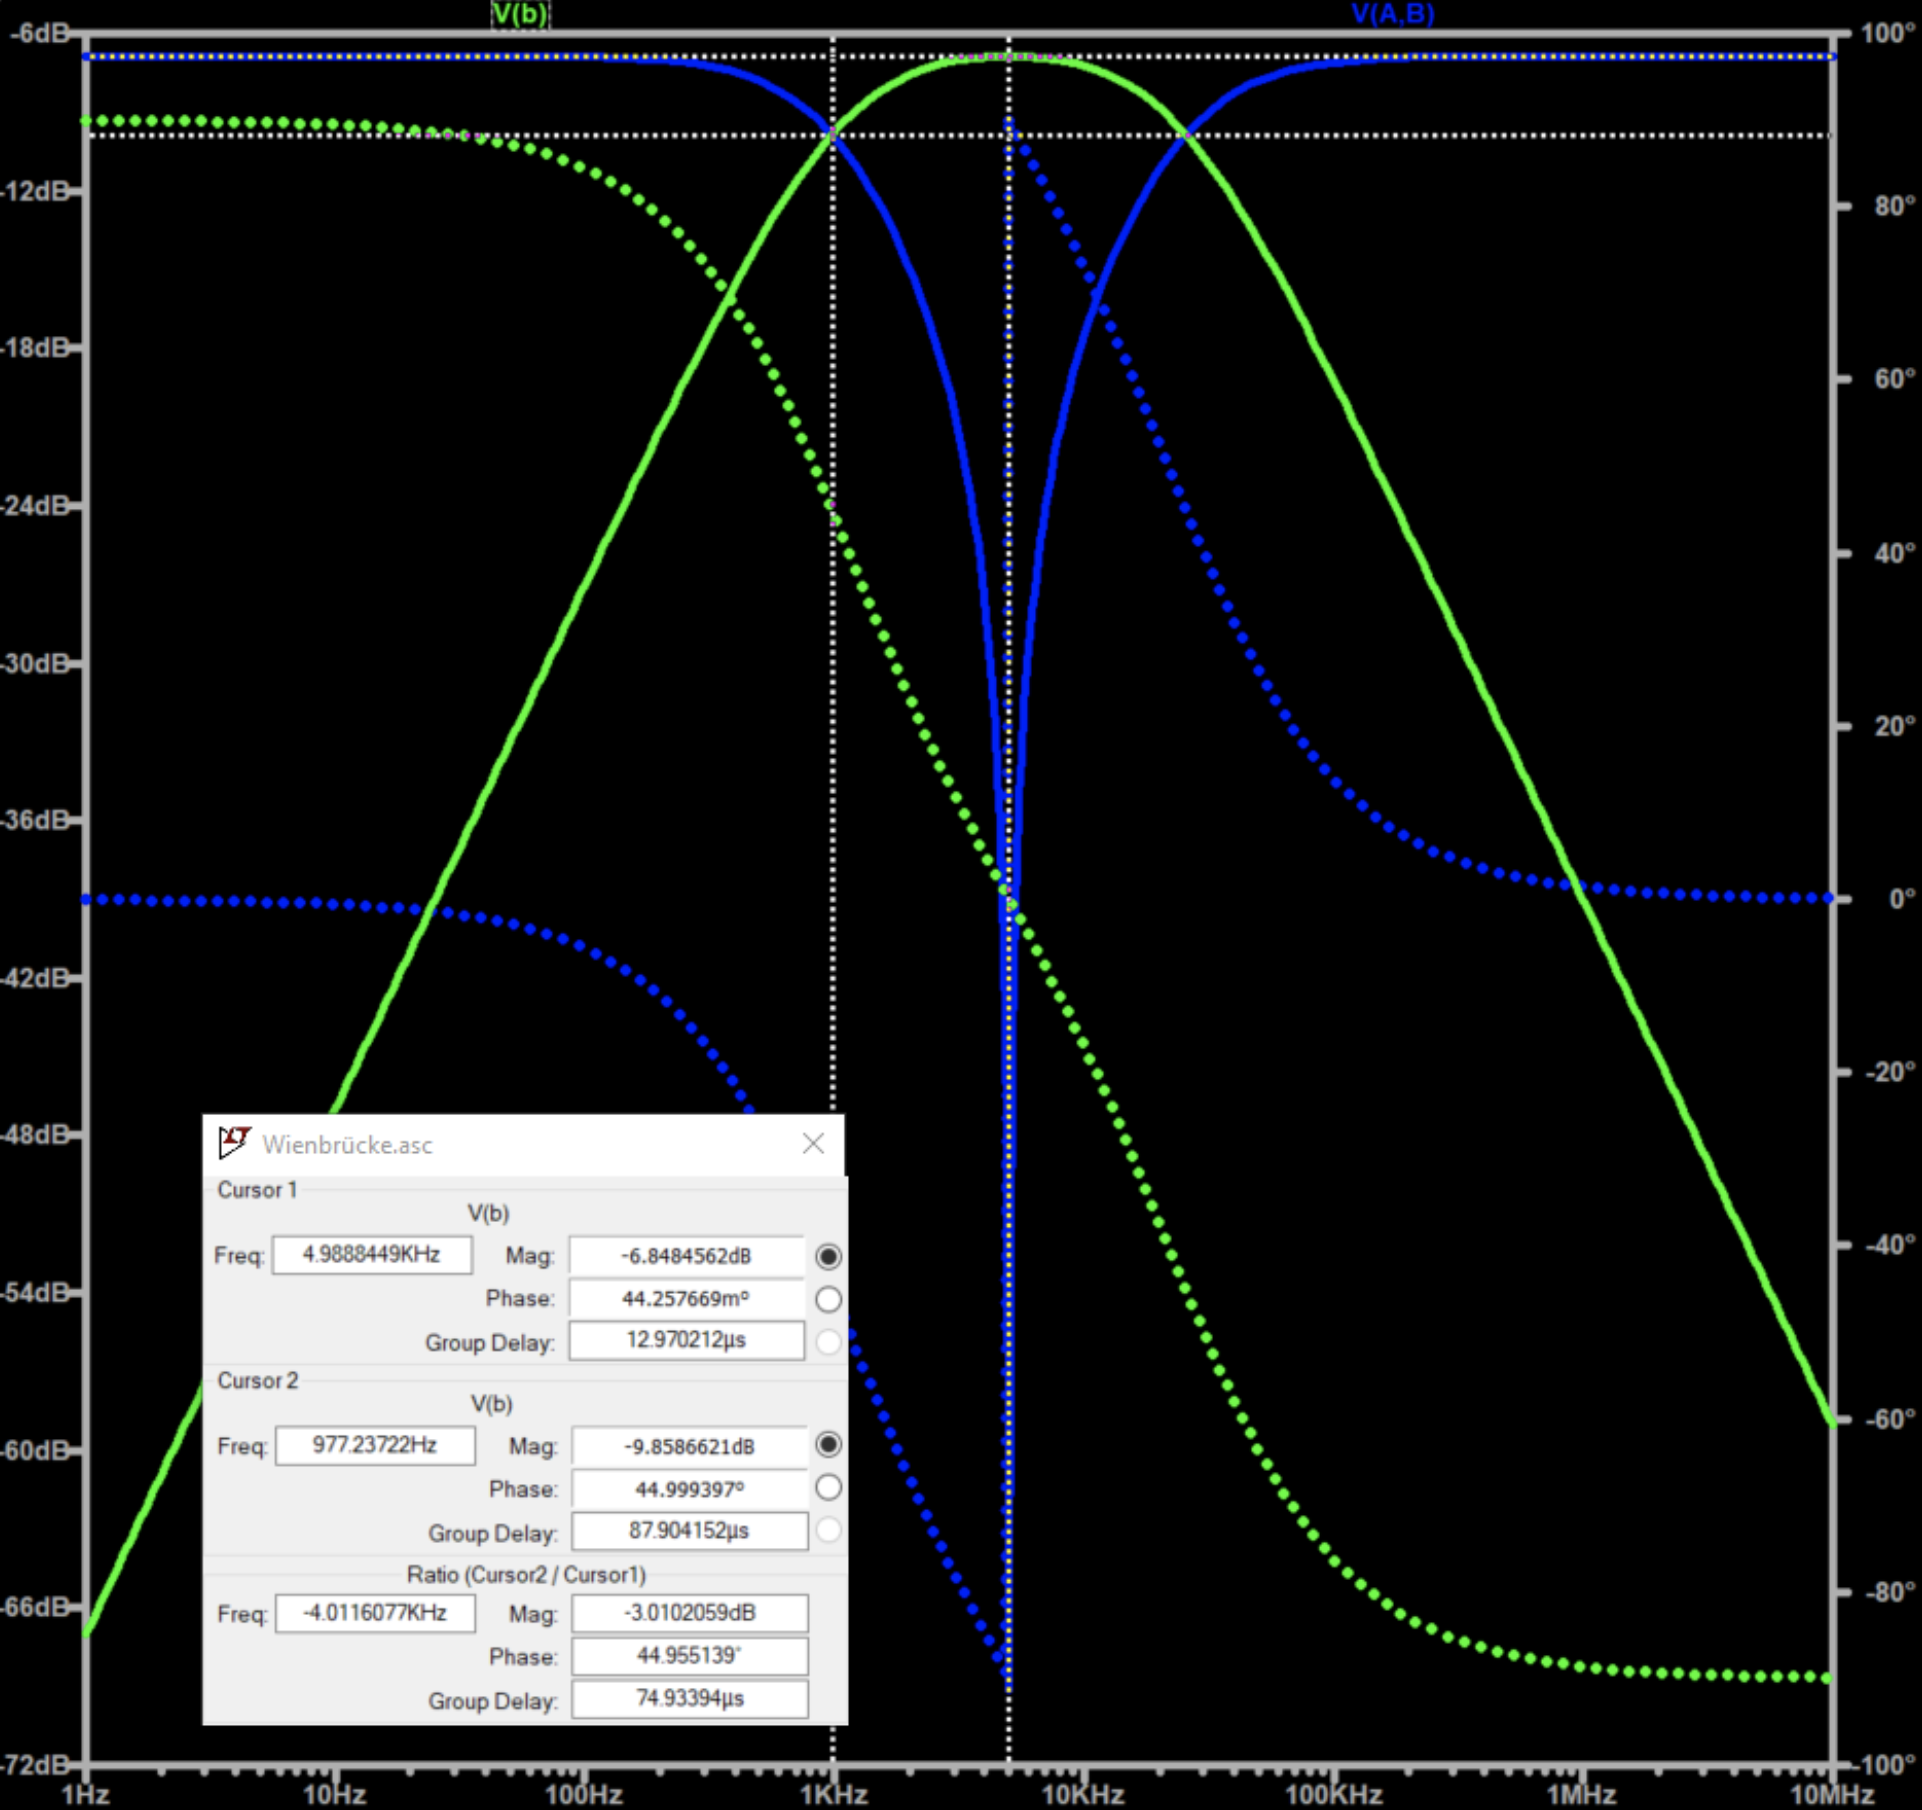
\includegraphics[width=4.5cm]{pictures/Bandsperre.png}}
  \end{figure}

\end{frame}

\begin{frame}[t]{Simulation - Abgleich mit Theorie}

  Bei einer Simulation ist es immer wichtig zu überprüfen, ob das Ergebnis durch eine theoretische Annahme verifiziert werden kann.
  Übernehmen wir nun die untere Grenzfrequenz $f_g=977Hz$ in unsere Spannungsquelle und betrachten nochmals den Zeitbereich über die transiente Simulation.

  \begin{spacing}{0.9} \begin{tiny}
      \begin{minipage}{\textwidth}
        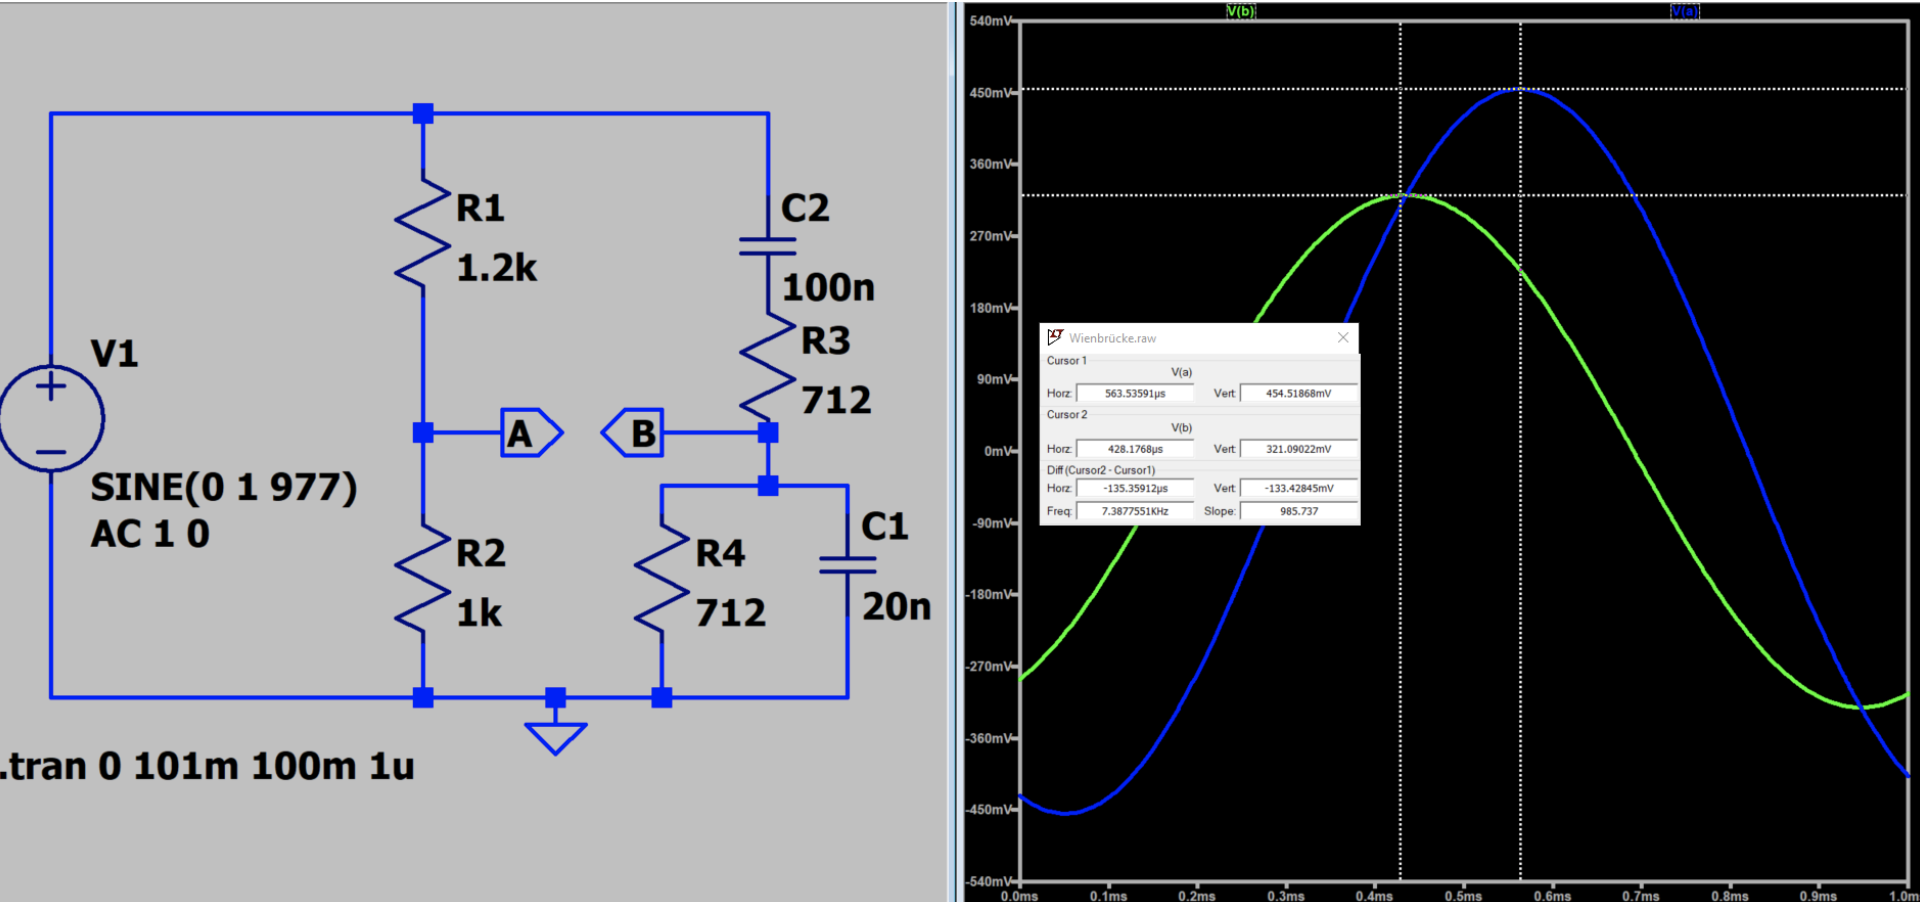
\includegraphics[width=0.75\linewidth]{pictures/wheatstone_transientent_fg.png}
      \end{minipage}
    \end{tiny} \end{spacing}

  \textbf{Das erwartete Verhalten bei der Grenzfrequenz $f_g$ ist, dass die Leistung auf $\frac{1}{\sqrt{2}}$ sinkt.}
\end{frame}

\begin{frame}[t]{Simulation - Abgleich mit Theorie}

  \begin{itemize}
    \item Wir können mittels der Cursor die Spannung $U_A=455mV$ und Spannung $U_B=321mV$ ermitteln.
    \item Dies stimmt mit unserer Erwartungshaltung überein.
  \end{itemize}
  \begin{figure}
    \centering
    $U_B=\frac{455mV}{\sqrt{2}}=321mV$
  \end{figure}

\end{frame}